

A cargo helicopter delivers only 100-pound packages and 120-pound packages. For each delivery trip, the helicopter must carry at least 10 packages, and the total weight of the packages can be at most 1,100 pounds. What is the maximum number of 120-pound packages that the helicopter can carry per trip?\\
A. 2\\
B. 4\\
C. 5\\
D. 6

\section*{ID: cfe67646}
The point $(8,2)$ in the $x y$-plane is a solution to which of the following systems of inequalities?\\
A. $x>0$\\
$y>0$\\
B. $x>0$\\
$y<0$\\
C. $x<0$\\
$y>0$\\
D. $x<0$\\
$y<0$

\section*{ID: 45cfb9de}
Adam's school is a 20-minute walk or a 5-minute bus ride away from his house. The bus runs once every 30 minutes, and the number of minutes, $w$, that Adam waits for the bus varies between 0 and 30 . Which of the following inequalities gives the values of $w$ for which it would be faster for Adam to walk to school?\\
A. $w-5<20$\\
B. $W-5>20$\\
C. $w+5<20$\\
D. $w+5>20$

\section*{ID: b1228811}
Marisa needs to hire at least 10 staff members for an upcoming project. The staff members will be made up of junior directors, who will be paid $\$ 640$ per week, and senior directors, who will be paid $\$ 880$ per week. Her budget for paying the staff members is no more than $\$ 9,700$ per week. She must hire at least 3 junior directors and at least 1 senior director. Which of the following systems of inequalities represents the conditions described if $x$ is the number of junior directors and $y$ is the number of senior directors?\\
$640 x+880 y \geq 9,700$\\
$x+y \leq 10$\\
$x \geq 3$\\
A. $y \geq 1$\\
$640 x+880 y \leq 9,700$\\
$x+y \geq 10$\\
$x \geq 3$\\
B. $y \geq 1$\\
$640 x+880 y \geq 9,700$\\
$x+y \geq 10$\\
$x \leq 3$\\
C. $y \leq 1$\\
$640 x+880 y \leq 9,700$\\
$x+y \leq 10$\\
$x \leq 3$\\
D. $y \leq 1$

\section*{ID: 2c121b25}
Valentina bought two containers of beads. In the first container 30\% of the beads are red, and in the second container $70 \%$ of the beads are red. Together, the containers have at least 400 red beads. Which inequality shows this relationship, where $x$ is the total number of beads in the first container and $y$ is the total number of beads in the second container?\\
A. $0.3 x+0.7 y \geq 400$\\
B. $0.7 x+0.3 y \leq 400$\\
C. $\frac{x}{3}+\frac{y}{7} \leq 400$\\
D. $30 x+70 y \geq 400$

\section*{ID: c50ede6d}
The total cost, in dollars, to rent a surfboard consists of a $\$ 25$ service fee and a $\$ 10$ per hour rental fee. A person rents a surfboard for $t$ hours and intends to spend a maximum of $\$ 75$ to rent the surfboard. Which inequality represents this situation?\\
A. $10 t \leq 75$\\
B. $10+25 t \leq 75$\\
C. $25 t \leq 75$\\
D. $25+10 t \leq 75$

In North America, the standard width of a parking space is at least 7.5 feet and no more than 9.0 feet. A restaurant owner recently resurfaced the restaurant's parking lot and wants to determine the number of parking spaces, $n$, in the parking lot that could be placed perpendicular to a curb that is 135 feet long, based on the standard width of a parking space. Which of the following describes all the possible values of $n$ ?\\
A. $18 \leq n \leq 135$\\
B. $7.5 \leq n \leq 9$\\
C. $15 \leq n \leq 135$\\
D. $15 \leq n \leq 18$

\section*{ID: 95cad55f}
A laundry service is buying detergent and fabric softener from its supplier. The supplier will deliver no more than 300 pounds in a shipment. Each container of detergent weighs 7.35 pounds, and each container of fabric softener weighs 6.2 pounds. The service wants to buy at least twice as many containers of detergent as containers of fabric softener. Let $d$ represent the number of containers of detergent, and let $s$ represent the number of containers of fabric softener, where $d$ and $s$ are nonnegative integers. Which of the following systems of inequalities best represents this situation?\\
A.\\
$7.35 d+6.2 s \leq 300$\\
$d \geq 2 s$\\
B.\\
$7.35 d+6.2 s \leq 300$\\
$2 d \geq s$\\
C.\\
$14.7 d+6.2 s \leq 300$\\
$d \geq 2 s$\\
$14.7 d+6.2 s \leq 300$\\
D.\\
$2 d \geq s$

$$
\begin{aligned}
& y \leq x \\
& y \leq-x
\end{aligned}
$$

Which of the following ordered pairs $(x, y)$ is a solution to the system of inequalities above?\\
A. $(1,0)$\\
B. $(-1,0)$\\
C. $(0,1)$\\
D. $(0,-1)$

\section*{ID: ee439cff}
On a car trip, Rhett and Jessica each drove for part of the trip, and the total distance they drove was under 220 miles. Rhett drove at an average speed of 35 miles per hour ( mph ), and Jessica drove at an average speed of 40 mph . Which of the following inequalities represents this situation, where $r$ is the number of hours Rhett drove and $j$ is the number of hours Jessica drove?\\
A. $35 r+40 j>220$\\
B. $35 r+40 j<220$\\
C. $40 r+35 j>220$\\
D. $40 r+35 j<220$



















































\section*{ID: ee7b1de1}
A small business owner budgets $\$ 2,200$ to purchase candles. The owner must purchase a minimum of 200 candles to maintain the discounted pricing. If the owner pays $\$ 4.90$ per candle to purchase small candles and $\$ 11.60$ per candle to purchase large candles, what is the maximum number of large candles the owner can purchase to stay within the budget and maintain the discounted pricing?

\section*{ID: c17d9ba9}
A number $x$ is at most 17 less than 5 times the value of $y$. If the value of $y$ is 3 , what is the greatest possible value of $x$ ?

\section*{ID: 1035faea}
A psychologist set up an experiment to study the tendency of a person to select the first item when presented with a series of items. In the experiment, 300 people were presented with a set of five pictures arranged in random order. Each person was asked to choose the most appealing picture. Of the first 150 participants, 36 chose the first picture in the set. Among the remaining 150 participants, p people chose the first picture in the set. If more than $20 \%$ of all participants chose the first picture in the set, which of the following inequalities best describes the possible values of $p$ ?\\
A. $p>0.20(300-36)$, where $p \leq 150$\\
B. $p>0.20(300+36)$, where $p \leq 150$\\
C. $p-36>0.20(300)$, where $p \leq 150$\\
D. $p+36>0.20(300)$, where $p \leq 150$

\section*{ID: 5bf5136d}
The triangle inequality theorem states that the sum of any two sides of a triangle must be greater than the length of the third side. If a triangle has side lengths of 6 and 12 , which inequality represents the possible lengths, $x$, of the third side of the triangle?\\
A. $x<18$\\
B. $x>18$\\
C. $6<x<18$\\
D. $x<6$ or $x>18$\\
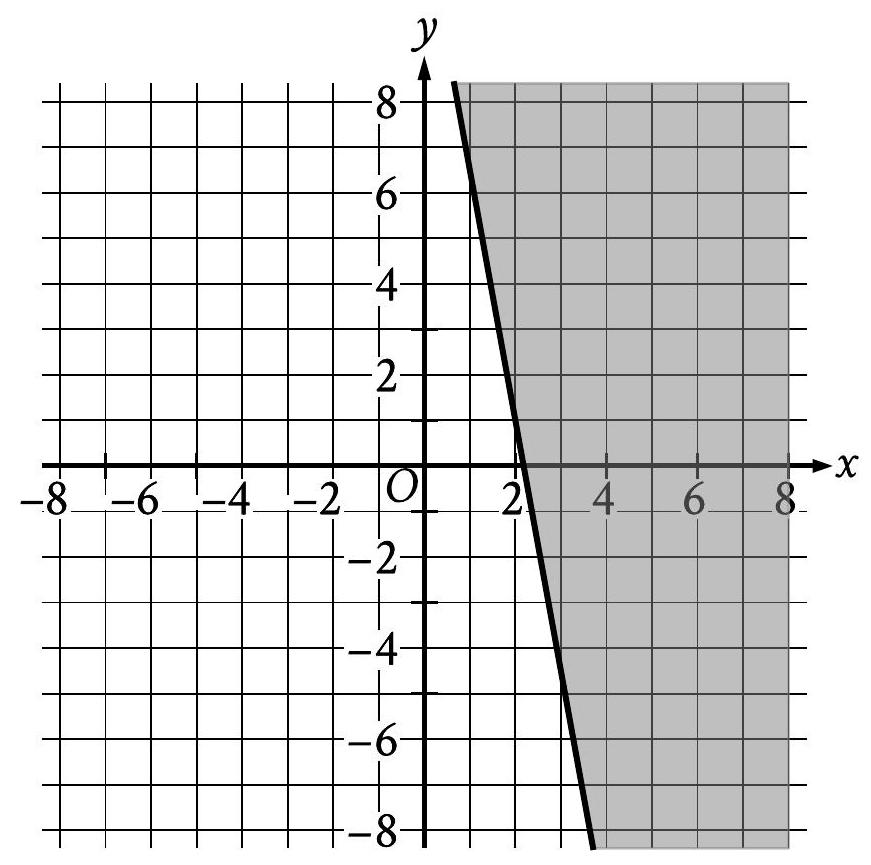
\includegraphics[max width=\textwidth, center]{2025_06_15_bde7e3e6a3b19d13464ag-25}

The shaded region shown represents solutions to an inequality. Which ordered pair $(x, y)$ is a solution to this inequality?\\
A. $(0,-4)$\\
B. $(0,4)$\\
C. $(-4,0)$\\
D. $(4,0)$

$$
\begin{gathered}
y>14 \\
4 x+y<18
\end{gathered}
$$

The point $(x, 53)$ is a solution to the system of inequalities in the $x y$-plane. Which of the following could be the value of $x$ ?\\
A. -9\\
B. -5\\
C. 5\\
D. 9

\section*{ID: e8f9e117}
$$
I=\frac{V}{R}
$$

The formula above is Ohm's law for an electric circuit with current $I$, in amperes, potential difference $V$, in volts, and resistance $R$, in ohms. A circuit has a resistance of 500 ohms, and its potential difference will be generated by $n$ six-volt batteries that produce a total potential difference of $6 n$ volts. If the circuit is to have a current of no more than 0.25 ampere, what is the greatest number, $n$, of six-volt batteries that can be used?

$$
y<6 x+2
$$

For which of the following tables are all the values of $x$ and their corresponding values of $y$ solutions to the given inequality?\\
A.

\begin{center}
\begin{tabular}{|c|c|}
\hline
$x$ & $y$ \\
\hline
3 & 20 \\
\hline
5 & 32 \\
\hline
7 & 44 \\
\hline
\end{tabular}
\end{center}

B.

\begin{center}
\begin{tabular}{|c|c|}
\hline
$x$ & $y$ \\
\hline
3 & 16 \\
\hline
5 & 36 \\
\hline
7 & 40 \\
\hline
\end{tabular}
\end{center}

c.

\begin{center}
\begin{tabular}{|c|c|}
\hline
$x$ & $y$ \\
\hline
3 & 16 \\
\hline
5 & 28 \\
\hline
7 & 40 \\
\hline
\end{tabular}
\end{center}

D.

\begin{center}
\begin{tabular}{|c|c|}
\hline
$x$ & $y$ \\
\hline
3 & 24 \\
\hline
5 & 36 \\
\hline
7 & 48 \\
\hline
\end{tabular}
\end{center}

$$
y>13 x-18
$$

For which of the following tables are all the values of $x$ and their corresponding values of $y$ solutions to the given inequality?\\
A.

\begin{center}
\begin{tabular}{|c|c|}
\hline
$x$ & $y$ \\
\hline
3 & 21 \\
\hline
5 & 47 \\
\hline
8 & 86 \\
\hline
\end{tabular}
\end{center}

B.

\begin{center}
\begin{tabular}{|c|c|}
\hline
$x$ & $y$ \\
\hline
3 & 26 \\
\hline
5 & 42 \\
\hline
8 & 86 \\
\hline
\end{tabular}
\end{center}

c.

\begin{center}
\begin{tabular}{|c|c|}
\hline
$x$ & $y$ \\
\hline
3 & 16 \\
\hline
5 & 42 \\
\hline
8 & 81 \\
\hline
\end{tabular}
\end{center}

D.

\begin{center}
\begin{tabular}{|c|c|}
\hline
$x$ & $y$ \\
\hline
3 & 26 \\
\hline
5 & 52 \\
\hline
8 & 91 \\
\hline
\end{tabular}
\end{center}

Normal body temperature for an adult is between $97.8^{\circ} \mathrm{F}$ and $99^{\circ} \mathrm{F}$, inclusive. If\\
Kevin, an adult male, has a body temperature that is considered to be normal, which of the following could be his body temperature?\\
A. $96.7^{\circ} \mathrm{F}$\\
B. $97.6^{\circ} \mathrm{F}$\\
C. $97.9^{\circ} \mathrm{F}$\\
D. $99.7^{\circ} \mathrm{F}$

Which of the following ordered pairs $(x, y)$ satisfies the inequality $5 x-3 y<4 ?$

\begin{enumerate}
  \item $(1,1)$
  \item $(2,5)$
  \item $(3,2)$\\
A. I only\\
B. II only\\
C. I and II only\\
D. I and III only
\end{enumerate}

\section*{ID: 84d0d07e}
A clothing store is having a sale on shirts and pants. During the sale, the cost of each shirt is $\$ 15$ and the cost of each pair of pants is $\$ 25$. Geoff can spend at most $\$ 120$ at the store. If Geoff buys shirts and p pairs of pants, which of the following must be true?\\
A. $15 s+25 p \leq 120$\\
B. $15 s+25 p \geq 120$\\
C. $25 s+15 p \leq 120$\\
D. $25 s+15 p \geq 120$

\section*{ID: 963da34c}
A shipping service restricts the dimensions of the boxes it will ship for a certain type of service. The restriction states that for boxes shaped like rectangular prisms, the sum of the perimeter of the base of the box and the height of the box cannot exceed 130 inches. The perimeter of the base is determined using the width and length of the box. If a box has a height of 60 inches and its length is 2.5 times the width, which inequality shows the allowable width $x$, in inches, of the box?\\
A. $0<x \leq 10$\\
B. $0<x \leq 11 \frac{2}{3}$\\
C. $0<x \leq 17 \frac{1}{2}$\\
D. $0<x \leq 20$

\section*{ID: 03503d49}
A business owner plans to purchase the same model of chair for each of the 81 employees. The total budget to spend on these chairs is $\$ 14,000$, which includes a $7 \%$ sales tax. Which of the following is closest to the maximum possible price per chair, before sales tax, the business owner could pay based on this budget?\\
A. $\$ 148.15$\\
B. $\$ 161.53$\\
C. $\$ 172.84$\\
D. $\$ 184.94$

\section*{ID: b8e73b5b}
Ken is working this summer as part of a crew on a farm. He earned $\$ 8$ per hour for the first 10 hours he worked this week. Because of his performance, his crew leader raised his salary to $\$ 10$ per hour for the rest of the week. Ken saves $90 \%$ of his earnings from each week. What is the least number of hours he must work the rest of the week to save at least $\$ 270$ for the week?\\
A. 38\\
B. 33\\
C. 22\\
D. 16

ID: 830120b0

$$
\begin{aligned}
y & >2 x-1 \\
2 x & >5
\end{aligned}
$$

Which of the following consists of the $y$-coordinates of all the points that satisfy the system of inequalities above?\\
A. $y>6$\\
B. $y>4$\\
C. $y>\frac{5}{2}$\\
D. $y>\frac{3}{2}$

\section*{ID: e744499e}
An elementary school teacher is ordering $x$ workbooks and $y$ sets of flash cards for a math class. The teacher must order at least 20 items, but the total cost of the order must not be over \$80. If the workbooks cost \$3 each and the flash cards cost \$4 per set, which of the following systems of inequalities models this situation?\\
A. 3

$$
x+y \geq 20
$$

$3 x+4 y \leq 80$\\
B. $\begin{aligned} x+y & \geq 20 \\ 3 x+4 y & \geq 80\end{aligned}$\\
$3 x+4 y \leq 20$\\
C.\\
$x+y \geq 80$\\
$x+y \leq 20$\\
D. $3 x+4 y \geq 80$

\section*{ID: 74c98c82}
An event planner is planning a party. It costs the event planner a onetime fee of $\$ 35$ to rent the venue and $\$ 10.25$ per attendee. The event planner has a budget of $\$ 200$. What is the greatest number of attendees possible without exceeding the budget?

\section*{ID: e9ef0e6b}
A model estimates that whales from the genus Eschrichtius travel 72 to 77 miles in the ocean each day during their migration. Based on this model, which inequality represents the estimated total number of miles, $x$, a whale from the genus Eschrichtius could travel in 16 days of its migration?\\
A. $72+16 \leq x \leq 77+16$\\
B. $(72)(16) \leq x \leq(77)(16)$\\
C. $72 \leq 16+x \leq 77$\\
D. $72 \leq 16 x \leq 77$

\section*{ID: f02b4509}
A moving truck can tow a trailer if the combined weight of the trailer and the boxes it contains is no more than 4,600 pounds. What is the maximum number of boxes this truck can tow in a trailer with a weight of 500 pounds if each box weighs 120 pounds?\\
A. 34\\
B. 35\\
C. 38\\
D. 39

\section*{ID: 90bd9ef8}
The average annual energy cost for a certain home is $\$ 4,334$. The homeowner plans to spend $\$ 25,000$ to install a geothermal heating system. The homeowner estimates that the average annual energy cost will then be $\$ 2,712$. Which of the following inequalities can be solved to find $t$, the number of years after installation at which the total amount of energy cost savings will exceed the installation cost?\\
A. $25,000>(4,334-2,712) t$\\
B. $25,000<(4,334-2,712) t$\\
C. $25,000-4,334>2,712 t$\\
D. $25,000>\frac{4,332}{2,712} t$

\section*{ID: 8f0c82e2}
The minimum value of $x$ is 12 less than 6 times another number $n$. Which inequality shows the possible values of $x$ ?\\
A. $x \leq 6 n-12$\\
B. $x \geq 6 n-12$\\
C. $x \leq 12-6 n$\\
D. $x \geq 12-6 n$

\section*{ID: b75f7812}
Maria plans to rent a boat. The boat rental costs $\$ 60$ per hour, and she will also have to pay for a water safety course that costs $\$ 10$. Maria wants to spend no more than $\$ 280$ for the rental and the course. If the boat rental is available only for a whole number of hours, what is the maximum number of hours for which Maria can rent the boat?\\
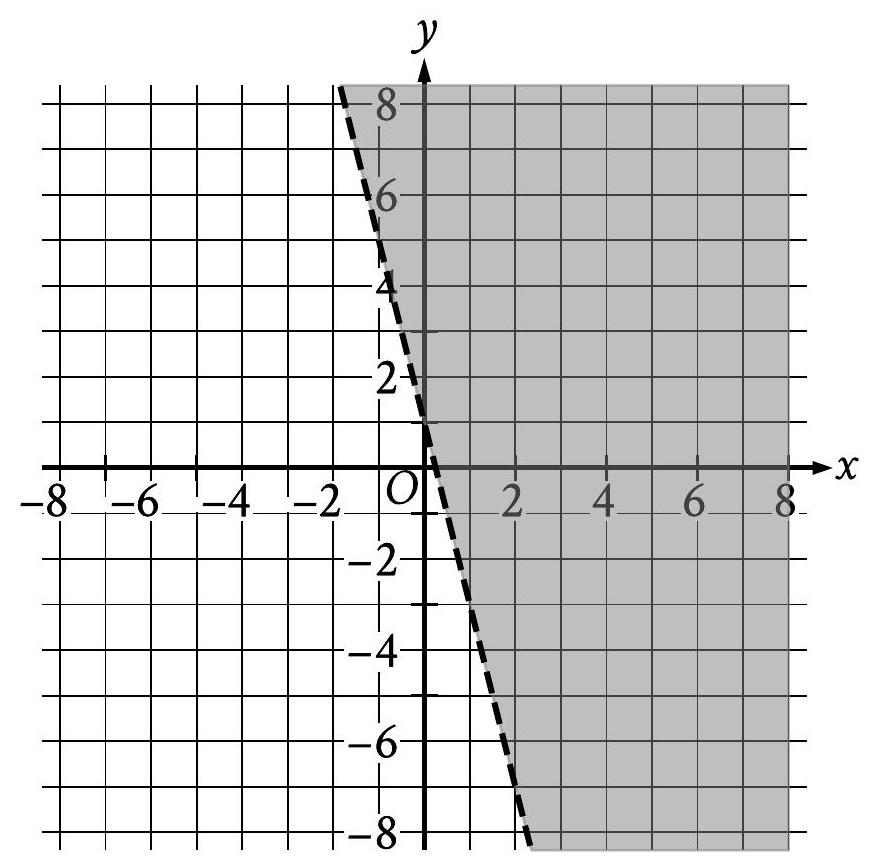
\includegraphics[max width=\textwidth, center]{2025_06_15_bde7e3e6a3b19d13464ag-44}

The shaded region shown represents the solutions to which inequality?\\
A. $y<1+4 x$\\
B. $y<1-4 x$\\
C. $y>1+4 x$\\
D. $y>1-4 x$

\section*{ID: b64e2c7f}
Monarch butterflies can fly only with a body temperature of at least 55.0 degrees Fahrenheit ( ${ }^{\circ} \mathrm{F}$ ). If a monarch butterfly's body temperature is $51.3^{\circ} \mathrm{F}$, what is the minimum increase needed in its body temperature, in ${ }^{\circ} \mathrm{F}$, so that it can fly?\\
A. 1.3\\
B. 3.7\\
C. 5.0\\
D. 6.3

\section*{ID: 7d6928bd}
A cleaning service that cleans both offices and homes can clean at most 14 places per day. Which inequality represents this situation, where $f$ is the number of offices and $h$ is the number of homes?\\
A. $f+h \leq 14$\\
B. $f+h \geq 14$\\
C. $f-h \leq 14$\\
D. $f-h \geq 14$

$$
\begin{array}{r}
y \leq 3 x+1 \\
x-y>1
\end{array}
$$

Which of the following ordered pairs ( $x, y$ ) satisfies the system of inequalities above?\\
A. $(-2,-1)$\\
B. $(-1,3)$\\
C. $(1,5)$\\
D. $(2,-1)$


